\chapter{Εισαγωγή στον Αντικειμενοστραφή Προγραμματισμό}
\label{chap:objects-intro}
\section{Εισαγωγή}
Ελπίζουμε να μη ζαλιστήκατε (πολύ) με τις τόσες νέες έννοιες στο προηγούμενο
κεφάλαιο! Αντικείμενα, συμβάντα, βιβλιοθήκη pygame, μέθοδοι, μέχρι
και\ldots{} φυσική Λυκείου είχαμε! Αλλά φυσικά μπρος στα\ldots{} graphics τι είναι ο
πόνος. Σίγουρα είστε διατεθειμένοι να κουραστείτε λίγο ακόμα -- εξάλλου
πλησιάζει η ώρα για το πρώτο μας πραγματικό γραφικό παιχνίδι. Και φυσικά,
δεν χρειάζεται να μας το πείτε: το ξέρουμε ότι είστε ήδη εθισμένοι με την
python, το προγραμματισμό, το pygame και όλα τα άλλα που ίσως δεν
πολυκαταλαβαίνετε ακόμα. Αλλά δεν πειράζει: το ξενύχτι είναι μέρος της
μαγείας! Πάμε λοιπόν να εξερευνήσουμε τον αντικειμενοστραφή
προγραμματισμό.

\section{Αντικειμενοστραφής Προγραμματισμός για\ldots{} Πρωτάρηδες}

Ή for Dummies θα λέγαμε αν κρατούσαμε τον Αγγλικό τίτλο της δημοφιλούς
σειράς βιβλίων Βέβαια οι αναγνώστες μας δεν είναι dummies -- κάθε άλλο
μάλιστα. Dummies είναι όσοι χρησιμοποιούν μόνο ετοιματζίδικα πράγματα!

Είναι σχετικά δύσκολο να πάρετε μια ικανοποιητική απάντηση στην ερώτηση
``Τι είναι αντικειμενοστραφής προγραμματισμός''. Είναι
μάλλον πιο εύκολο να το δει κανείς στα προγράμματα παρά να προσπαθεί με
ένα θεωρητικό ορισμό. Ωστόσο οι περισσότεροι συμφωνούμε στα παρακάτω:

\begin{description}
 \item[Αντικείμενο:] Είναι μια συλλογή από δεδομένα --- μπορείτε
    να τα πείτε {\em χαρακτηριστικά (attributes)}, {\em ιδιότητες (properties)} --- με την
    ιδιαιτερότητα ότι έχει τις δικές του συναρτήσεις ({\em μεθόδους})
    για να τα χειρίζεται.

Για να δημιουργήσουμε  δικά μας αντικείμενα (που να περιέχουν τα
    δεδομένα και τις μεθόδους της επιλογής μας) γράφουμε μια
    {\em κλάση}. Σε αυτή περιγράφουμε τα δεδομένα που θα περιέχει
    το αντικείμενο μας καθώς και τις μεθόδους που τα χειρίζονται. Όταν
    δημιουργήσουμε ένα αντικείμενο που ανήκει στην κλάση μας, αυτόματα θα
    διαθέτει τα χαρακτηριστικά και τις μεθόδους που ορίσαμε.

Δεν είναι όμως μόνο αυτό. Στο κάτω -- κάτω θα μπορούσατε να σκεφτείτε ότι
    δεν αλλάζει κάτι ιδιαίτερα: Αντί να έχουμε συναρτήσεις και να τους δίνουμε
    τα δεδομένα μας, τα ίδια τα δεδομένα μας έχουν τις δικές τους συναρτήσεις.
    Ε και λοιπόν; Ο αντικειμενοστραφής προγραμματισμός έχει ακόμα τρεις
    βασικές έννοιες:

	 \item[Πολυμορφία (polymorphism):] Φανταστείτε δύο
	 αντικείμενα από διαφορετικές κλάσεις να διαθέτουν μια μέθοδο με το
	 ίδιο όνομα. Ανάλογα με το αντικείμενο που χρησιμοποιείται όταν
	 γίνεται η κλήση, καλείται κάθε φορά η σωστή μέθοδος!
	 \item[Ενθυλάκωση (encapsulation):] Άλλο πράγμα
	 να γράψεις πως δουλεύει ένα αντικείμενο (στο κομμάτι που περιγράφεται
	 η κλάση) και άλλο να το χρησιμοποιείς μετά για το κανονικό σου
	 πρόγραμμα. Στη χρήση, δεν μας ενδιαφέρει πλέον πως λειτουργεί
	 εσωτερικά το αντικείμενο, αρκεί να κάνει αυτό που θέλουμε. Η
	 ενθυλάκωση κρύβει την εσωτερική πολυπλοκότητα του αντικειμένου
	 όταν πλέον δεν χρειάζεται να την βλέπουμε. Σκεφτείτε το και ως εξής:
	 Δεν ξέρετε πως λειτουργεί εσωτερικά η επιφάνεια
	 (surface) του pygame. Μπορείτε όμως να τη χρησιμοποιήσετε
 	 γιατί το μόνο που χρειάζεστε να ξέρετε είναι οι λειτουργίες που
	 σας παρέχουν οι μέθοδοι.
	 \item[Κληρονομικότητα (inheritance):] Με αυτήν
	 την καταπληκτική δυνατότητα μπορείτε να ξεκινήσετε δημιουργώντας μια
	 γενική κλάση αντικειμένων και από αυτή να παράγετε πιο εξειδικευμένες
	 κλάσεις με πρόσθετα χαρακτηριστικά που να κληρονομούν όμως και τα
	 χαρακτηριστικά και τις μεθόδους της γονικής τους κλάσης.
\end{description}

Ειδικά η κληρονομικότητα σε συνδυασμό με την πολυμορφία μας επιτρέπουν να
κάνουμε ιδιαίτερα καλά κόλπα. Όμως αντί να σας τα λέμε θεωρητικά, θα σας
τα δείξουμε με παραδείγματα. Όχι τίποτα άλλο δηλαδή, αλλά κάποιοι από εσάς
αναμφίβολα μένετε σε\ldots{} ψηλούς ορόφους και δεν μπορούμε να συνεχίσουμε άλλο
τη θεωρία. Και πραγματικά, αν κάπου μας χάσατε με τα παραπάνω μην ανησυχείτε:
όλα θα ξεκαθαρίσουν στην πορεία.

\section{Θεός για\ldots{} μια Ημέρα!}

Φανταστείτε ότι είστε ο\ldots{} θεός και πρόκειται να δημιουργήσετε τη ζωή πάνω
στη Γη. Σε python βέβαια! Έχετε ήδη ασχοληθεί με φυτά και άλλα τέτοια\ldots{}
βαρετά, και έχετε φτάσει στα θηλαστικά. Σκέφτεστε λοιπόν να φτιάξετε μια
κλάση θηλαστικών και από αυτή να παράγετε ότι άλλο χρειάζεστε (γάτες,
σκύλους, ανθρώπους and so on). Προφανώς ένα αντικείμενο που ανήκει σε μια
τέτοια κλάση έχει διάφορα χαρακτηριστικά (attributes) και λειτουργίες
(μεθόδους) αλλά για το παράδειγμα μας θα επικεντρωθούμε σε ένα: την
ομιλία.

Όλα τα θηλαστικά έχουν κάποιο είδος φωνής: οι σκύλοι γαβγίζουν (bark), οι
γάτες νιαουρίζουν (meow), ε και οι άνθρωποι\ldots{} μερικές φορές καλύτερα να
μασάνε παρά να μιλάνε. Καθώς φαντάζεστε, σαν θεός θα πρέπει να φτιάξετε
μια μέθοδο {\tt speak} που όταν την καλείτε να κάνει το σωστό, ανάλογα με το
ζώο. Στο κάτω κάτω δεν υπάρχουν σκύλοι που να νιαουρίζουν και γάτες που
να γαβγίζουν!

Ξεκινάτε δημιουργώντας μια κλάση που περιγράφει τα θηλαστικά γενικά:

\begin{minted}[bgcolor=bg, frame=lines, framesep=10pt]{python}
class mammal:
  def speak(self):
    print "Mpla mpla!"
\end{minted}

Η δημιουργία μιας κλάσης ξεκινάει με την εντολή {\tt class}. Για να γράψουμε μια
μέθοδο που ανήκει στην κλάση, την γράφουμε ως συνάρτηση (με την {\tt def} που
ξέρουμε ήδη) μέσα στην κλάση. Το {\tt self} που βλέπετε σημαίνει ότι το πρώτο
όρισμα της συνάρτησης είναι ένα αντικείμενο της ίδιας της κλάσης που ορίζουμε.

Μπορείτε τώρα να δημιουργήσετε ένα ζώο της γενικής κατηγορίας {\tt mammal} και να το βάλετε να μιλήσει. Όταν δημιουργούμε ένα αντικείμενο που ανήκει σε μια
κλάση λέμε ότι έχουμε φτιάξει ένα {\em instance} αυτής της κλάσης:

\begin{minted}[bgcolor=bg, frame=lines, framesep=10pt]{python}
animal = mammal()
animal.speak()
\end{minted}

Το οποίο βέβαια θα σας τυπώσει:

\begin{verbatim}
Mpla mpla!
\end{verbatim}

Βέβαια εμείς δεν ξέρουμε κανένα ζώο να έχει για φωνή το μπλα μπλα, οπότε
θα φτιάξουμε τώρα την ειδική κλάση γάτας και σκύλου, η οποία προέρχεται
από τη {\tt mammal}:

\begin{minted}[bgcolor=bg, linenos, frame=lines, framesep=10pt]{python}
class cat(mammal):
  def speak(self):
    print "Meow!"

class dog(mammal):
  def speak(self):
    print "Bark!"

# Δημιουργία γάτας!

thecat = cat()

# Δημιουργία σκύλου!

thedog = dog()

# Ομιλία!

thecat.speak()
thedog.speak()
\end{minted}

Φτιάξαμε μια κλάση {\tt cat} και μια {\tt dog} που προέρχονται από τη {\tt
mammal} (το δηλώσαμε αυτό γράφοντας το όνομα της γονικής κλάσης μέσα στην παρένθεση) αλλά καθεμιά από αυτές υλοποιεί ξανά τη μέθοδο {\tt speak}. Έτσι μια γάτα όταν καλούμε τη μέθοδο {\tt speak} δεν λέει μπλα μπλα, αλλά meow και ένας σκύλος bark! Τώρα είμαι σίγουρος ότι αν ο γείτονας σας έχει σκύλο που γαβγίζει κάθε βράδυ, ξέρετε ποια είναι η λύση: Να του γράψετε μια μέθοδο {\tt shutup} και να την καλέσετε!

Συνήθως δίνουμε ονόματα στις γάτες και τους σκύλους μας, οπότε σαν θεός που
είστε θέλετε να το προβλέψετε αυτό στην κλάση σας. Κανένα πρόβλημα. Μόνο
που δεν χρειάζεται να το γράψετε χωριστά για το σκύλο και τη γάτα. Βάλτε το
απλώς στην κλάση {\tt mammal} και θα το κληρονομήσουν:

\begin{minted}[bgcolor=bg, linenos, frame=lines, framesep=10pt]{python}
class mammal:
  def speak(self):
    print "Mpla mpla!"
  def setName(self, name):
    self.name = name
  def getName(self):
    return self.name
\end{minted}

Δοκιμάστε προσθέτοντας τις παρακάτω γραμμές στο κύριο πρόγραμμα:

\begin{minted}[bgcolor=bg, linenos, frame=lines, framesep=10pt]{python}
thecat.setName("Catia")
thedog.setName("Lassie")
print thecat.getName()
print thedog.getName()
\end{minted}

Μπορούμε επίσης να έχουμε απευθείας πρόσβαση στα δεδομένα της κλάσης,
χωρίς να χρησιμοποιήσουμε τις συναρτήσεις {\tt getName} και {\tt setName} που
φτιάξαμε:

\begin{minted}[bgcolor=bg, frame=lines, framesep=10pt]{python}
print thedog.name
thecat.name="Susan"
print thecat.name
\end{minted}

Σε πολλές περιπτώσεις, όταν δημιουργούμε ένα αντικείμενο θέλουμε να έχει
από την αρχή κάποια δεδομένα ή ιδιότητες. Για παράδειγμα, σαν θεός
αποφασίσατε ότι όλες οι γάτες θα γεννιούνται\ldots{} μαύρες και όλα τα θηλαστικά
θα έχουν τέσσερα πόδια! Για να δώσετε αρχική κατάσταση σε ένα αντικείμενο
κατά τη δημιουργία του, χρειάζεστε μια ειδική συνάρτηση που ονομάζεται
{\em constructor}. Για το παράδειγμα μας:

\begin{minted}[bgcolor=bg, linenos, frame=lines, framesep=10pt]{python}
class mammal(object):
  def __init__(self):
    self.legs=4
  def speak(self):
    print "Mpla mpla!"
  def setName(self, name):
    self.name = name
  def getName(self):
    return self.name

class cat(mammal):
  def __init__(self):
    super(cat,self).__init__()
    self.color="black"
  def speak(self):
    print "Meow!"

thecat = cat()
print thecat.color
print thecat.legs
\end{minted}

Προσέξτε τη συνάρτηση {\tt \_\_init\_\_} στην κλάση {\tt mammal}: Ορίζει ότι όλα τα
θηλαστικά έχουν\ldots{} τέσσερα πόδια. (Θεός είστε ότι θέλετε κάνετε.)
Αντίστοιχα, ο constructor για τις γάτες ορίζει ότι το χρώμα τους θα είναι
μαύρο.

Με μια προσεκτικότερη ματιά, θα δείτε ότι το class {\tt mammal} φαίνεται να
προέρχεται πλέον από την γενικότερη κλάση object. Αυτό το χρειαζόμαστε για να λειτουργήσει η συνάρτηση {\tt super} στον constructor της γάτας -- και θα
δούμε τώρα τι κάνει αυτή.

Όταν δημιουργείτε μια γάτα, καλείται ο constructor στην κλάση της. Προσέξτε
ότι δεν καλείται ο constructor του {\tt mammal}, όχι αυτόματα δηλαδή. Σε κάποιες
γλώσσες, όταν δημιουργούμε ένα αντικείμενο μιας {\em υποκλάσης (subclass)},
καλείται πρώτα αυτόματα ο constructor της {\em γονικής κλάσης (superclass)}.
Στην python αυτό δεν συμβαίνει. Θα πρέπει αν θέλουμε να καλέσουμε τον
constructor της mammal να το κάνουμε μέσα από τον constructor της cat.
Θα μπορούσε να γίνει ως εξής:

\begin{minted}[bgcolor=bg, frame=lines, framesep=10pt]{python}
mammal.__init__(self)
\end{minted}

Αλλά ο νέος Σωστός Τρόπος\texttrademark{} είναι:

\begin{minted}[bgcolor=bg, frame=lines, framesep=10pt]{python}
super(cat,self).__init__()
\end{minted}

Με την {\tt super} ουσιαστικά λέμε να χρησιμοποιηθεί η κλάση από την οποία
προέρχεται η {\tt cat} (δηλ. η {\tt mammal}).

\section{Ένα Αντικειμενοστραφές\ldots{} Bouncing Ball}

Στο προηγούμενο κεφάλαιο, σας δώσαμε ένα μάλλον κακογραμμένο κομμάτι κώδικα το
το οποίο υλοποιούσε ένα bouncing ball με δύο μπάλες. Όπως διαπιστώσατε
δεν είχε σημαντικές διαφορές με το πρωτότυπο. Γιατί απλά, για δύο μπάλες
χρειάζεστε:

\begin{itemize}
  \item Το ίδιο γραφικό δύο φορές. Εύκολο, το έχουμε ήδη.
  \item Διπλές μεταβλητές που δείχνουν: θέση μπάλας, απόσταση που διανύθηκε,
      ταχύτητα σε κάθε άξονα.
\end{itemize}

Αν προσέξετε λοιπόν το listing θα διαπιστώσετε ότι οι μεταβλητές για τη
μια μπάλα\ldots{} κλωνοποιούνται για τη δεύτερη:

\begin{itemize}
  \item[-] Θέση πρώτης μπάλας: μεταβλητές {\tt x} και {\tt y}. Θέση δεύτερης μπάλας: {\tt x2} και {\tt y2}
  \item[-] Ταχύτητα πρώτης μπάλας: {\tt xspeed} και {\tt yspeed}, δεύτερης μπάλας {\tt xspeed2} και {\tt yspeed2}
  \item[-] Απόσταση που διάνυσε η πρώτη μπάλα: {\tt distance\_x} και {\tt distance\_y}, δεύτερη μπάλα {\tt distance\_x2} και {\tt distance\_y2}
\end{itemize}

Αν και μπορεί αρχικά να σας φάνηκε ικανοποιητική η λύση, σίγουρα
κολλήσατε όταν σας ζητήσαμε να το φτιάξετε για τρεις, πέντε, δέκα μπάλες.
Όχι ότι δεν γίνεται να συνεχίσετε να προσθέτετε μεταβλητές, αλλά είναι
προφανές ότι η λύση αυτή δεν είναι ούτε κομψή ούτε γενική. Τι θα
μπορούσατε να σκεφτείτε;

Έχετε καταλάβει σίγουρα ότι όταν έχουμε δεδομένα ίδιου τύπου, που θέλουμε
να τα χειριστούμε μαζικά με τον ίδιο τρόπο, βολεύει αντί να τα
αποθηκεύσουμε σε απλές μεταβλητές να χρησιμοποιήσουμε κάποια δομή που μας
παρέχει η γλώσσα προγραμματισμού μας για αυτό το σκοπό. Για παράδειγμα,
οι παραδοσιακές γλώσσες (όπως η BASIC από την οποία άλλωστε προέρχεται
και το αρχικό μας bouncing ball) χρησιμοποιούν πίνακες. Στην python όπως
θα έχετε καταλάβει βασική δομή για αυτό το σκοπό είναι οι λίστες.

Οι λίστες όπως και οι πίνακες μας επιτρέπουν μαζική επεξεργασία των
δεδομένων καθώς μας επιτρέπουν να εκτελέσουμε σε κάθε στοιχείο τους την
ίδια λειτουργία, διατρέχοντας τα με κάποιο βρόχο. Πράγματι μια πιθανή λύση θα ήταν να δημιουργούσαμε μια λίστα που να περιέχει μέσα τις
τιμές των στοιχείων:

\begin{minted}[bgcolor=bg, frame=lines, framesep=10pt]{python}
[x, y, xspeed, yspeed]
\end{minted}

Επειδή μάλιστα θα χρειαζόμασταν μια τέτοια για κάθε μπάλα, θα είχαμε
πολλές τέτοιες λίστες μέσα σε μια άλλη (αυτό δεν είναι κάτι καινούριο,
θυμηθείτε το έχουμε κάνει στο Adventure). Π.χ.:

\begin{minted}[bgcolor=bg, frame=lines, framesep=10pt]{python}
balls = [ [100.0, 100.0, 50.0,50.0],
          [50.0, 50.0, 30.0, 30.0], ...]
\end{minted}

Πράγματι έτσι το πρόγραμμα μας θα γίνονταν αμέσως πολύ καλύτερο: Αντί να
γράφουμε συνέχεια τις ίδιες εντολές με άλλα ονόματα μεταβλητών, θα είχαμε
ένα βρόχο {\tt for} που θα διέτρεχε τη λίστα, και θα εκτελούσε τις εντολές σε
κάθε στοιχείο χωριστά. Μια χαρά.

Μια χαρά, μόνο που δεν είμαστε στα 80s! Είπαμε να εμπνευστούμε από τα
προγράμματα του TI-99/4A, όχι να τα ξαναγράψουμε στη BASIC της εποχής!
Ο κόσμος μας φωνάζει απεγνωσμένα ότι θέλει να γίνει object oriented!

Τι είναι μια μπάλα σαν αντικείμενο; Δείτε:
\begin{SCfigure}
  \centering
  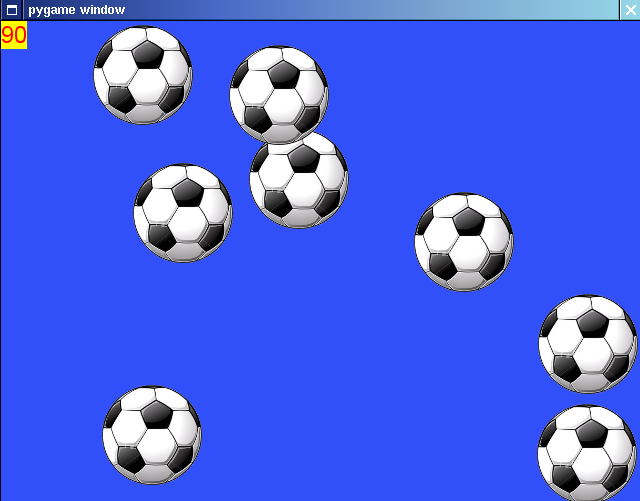
\includegraphics[width=0.43\textwidth]{images/chapter5/bouncing-ball-oop}
  \caption[Αντικειμενοστραφές Bouncing Ball]{Το αντικειμενοστραφές Bouncing
Ball δεν έχει κανένα πρόβλημα στο πόσες μπάλες θα δείξει! (από την άλλη ίσως
έχει πρόβλημα το σαράβαλο που χρησιμοποιείτε για υπολογιστή. Χμμμ\ldots{}) Μάλιστα το μόνο που χρειάζεται είναι να αλλάξετε ένα αριθμό στον κώδικα. Ποιο;}
  \label{5-1}
\end{SCfigure}

\begin{minted}[bgcolor=bg,linenos, frame=lines, framesep=10pt]{python}
import pygame
from pygame.locals import *
import random
from sys import exit
\end{minted}

\begin{minted}[bgcolor=bg, firstnumber=5, linenos, frame=lines, framesep=10pt]{python}
class Ball:
  def __init__(self,theImage,x,y,xspeed,yspeed):
    self.ballimage = theImage
    self.x = x
    self.y = y
    self.xspeed = xspeed
    self.yspeed = yspeed
    self.shape = pygame.image.load(theImage)

  def Show(self,surface):
    surface.blit(self.shape, (self.x, self.y))
\end{minted}

\begin{minted}[bgcolor=bg,linenos, firstnumber=16, frame=lines, framesep=10pt]{python}
  def GetWidth(self):
    return self.shape.get_width()

  def GetHeight(self):
    return self.shape.get_height()

  def Move(self, time):
    distance_x = time * self.xspeed
    distance_y = time * self.yspeed
    self.x = self.x + distance_x
    self.y = self.y + distance_y

  def IsOutofX(self,xmin,xmax):
    if (self.x >= (xmax - self.GetWidth()) or self.x <= xmin):
      return True
    else:
      return False

  def IsOutofY(self,ymin,ymax):
    if (self.y >= (ymax - self.GetHeight()) or self.y <= ymin):
      return True
    else:
      return False
\end{minted}

Μη φωνάζετε! Είναι απλούστατο: Η μπάλα για τον εαυτό της κρατάει τις
πληροφορίες που είπαμε πριν: Θέση ({\tt x} και {\tt y}), ταχύτητα ({\tt
xspeed} και {\tt yspeed}) και την εικόνα (hint: όχι μόνο μπορείτε να φτιάξετε πολλαπλά bouncing balls, αλλά κάθε μπάλα να έχει και δική της μορφή). Δείτε λίγο
τον constructor, τη συνάρτηση δημιουργίας ενός αντικειμένου τύπου
μπάλας:

\begin{minted}[bgcolor=bg, frame=lines, framesep=10pt]{python}
  def __init__(self,theImage,x,y,xspeed,yspeed):
\end{minted}

O συγκεκριμένος constructor παίρνει και κάποιες αρχικές τιμές οι
οποίες αποδίδονται απευθείας στις μεταβλητές ιδιοτήτων της μπάλας μας.
Τυπικά, για να δημιουργήσουμε μια μπάλα στο κύριο πρόγραμμα μας, θα
γράψουμε κάτι σαν το παρακάτω:

\begin{minted}[bgcolor=bg, frame=lines, framesep=10pt]{python}
MyBall = Ball("soccer.png",100.0,100.0,50.0,50.0)
\end{minted}

Φυσικά εννοείτε ότι αντί για απευθείας (literal) τιμές, θα μπορούσαμε
εδώ να έχουμε μεταβλητές. Αλλά για να δούμε τι άλλες συναρτήσεις
περιέχει η κλάση μας -- με λίγα λόγια τι ξέρει να κάνει η μπάλα μας από
μόνη της:

\begin{minted}[bgcolor=bg, frame=lines, framesep=10pt]{python}
def Show(self,surface):
\end{minted}

Να δείξει τον εαυτό της σε μια επιφάνεια που θα της δώσουμε (με τη μέθοδο
blit φυσικά)

\begin{minted}[bgcolor=bg, frame=lines, framesep=10pt]{python}
def GetWidth(self):
def GetHeight(self):
\end{minted}

Να μας πει το μέγεθος της (πλάτος και ύψος) σε pixels χρησιμοποιώντας το
{\tt get\_width} και {\tt get\_height} του pygame.

\begin{minted}[bgcolor=bg, frame=lines, framesep=10pt]{python}
def Move(self,time):
\end{minted}

Να κινηθεί. Πολύ λογικό: γνωρίζει τόσο την ταχύτητα της --- όπως τη δώσαμε
στον constructor --- όσο και τις προηγούμενες συντεταγμένες της. Οπότε το
μόνο που χρειάζεται για τον υπολογισμό είναι και ο χρόνος που περνάμε ως
παράμετρο από το κύριο πρόγραμμα.

\begin{minted}[bgcolor=bg, frame=lines, framesep=10pt]{python}
def IsOutofX(self, xmin, xmax):
def IsOutofY(self, ymin, ymax):
\end{minted}

Να ελέγξει αν έχει βγει εκτός ορίων της οθόνης, σε οποιοδήποτε από τους
δύο άξονες. Το μόνο έξτρα που χρειάζεται είναι φυσικά τα ίδια τα όρια,
τα οποία και πάλι τα περνάμε ως παραμέτρους.

Από εκεί και πέρα το πρόγραμμα είναι πολύ απλό.
Θα διαπιστώσετε ότι χρησιμοποιούμε μια λίστα που αποθηκεύει\ldots{} μπάλες.
Στην κυριολεξία, η λίστα αυτή περιέχει μέσα αντικείμενα τύπου μπάλας,
τα οποία προσθέτουμε με τον τρόπο που φαίνεται παρακάτω:

\begin{minted}[bgcolor=bg, frame=lines, framesep=10pt]{python}
balls=[]
for i in range(0,8):
  balls.append(Ball(ballimage,x,y,xspeed,yspeed))
\end{minted}

Βλέπετε βέβαια την απλή εκδοχή, γιατί μέσα στο βρόχο υπάρχουν και εντολές
που δημιουργούν για κάθε μπάλα νέες τυχαίες τιμές θέσης και ταχύτητας.
Δείτε και το υπόλοιπο πρόγραμμα και θα το καταλάβετε αμέσως.

\begin{minted}[bgcolor=bg, linenos, frame=lines, framesep=10pt]{python}
def getQuit():
  for event in pygame.event.get():
    if event.type == QUIT:
      return True
  return False

def main():
  pygame.init()
  ballimage = 'soccer-ball.png'
  balls=[]
  for i in range(0,8):
    x = random.randint(80,500)
    y = random.randint(80,400)
    xspeed = 0
    while (xspeed >= -5 and xspeed <= 5):
      xspeed = random.randint(-50,50)
    yspeed = 0
\end{minted}

\begin{minted}[bgcolor=bg, linenos, firstnumber=18, frame=lines, framesep=10pt]{python}
    while (yspeed >= -5 and yspeed <=5):
      yspeed = random.randint(-50,50)
    balls.append(Ball(ballimage,x,y,xspeed,yspeed))
  windowsize = (640,480)
  surfacecolor = (50,80,250)
  screen = pygame.display.set_mode(windowsize, DOUBLEBUF)
  clock = pygame.time.Clock()

  # Uncomment the framerate line and change
  # time = clock.tick() in main loop to
  # time = clock.tick(framerate)
  # to limit the animation to a specific framerate

  #framerate = 30

  textfont = pygame.font.SysFont("Arial",24)
  #
  # Main loop
  #

  endprogram = False
  while not endprogram:
    screen.fill(surfacecolor)
    for theball in balls:
      theball.Show(screen)
    time = clock.tick()
    thetext = textfont.render(str(1000/time), True, (255,0,0),(255,255,0))
    screen.blit(thetext,(0,0))
    time = time / 1000.0
\end{minted}

\begin{minted}[bgcolor=bg, linenos, firstnumber=47, frame=lines, framesep=10pt]{python}
    for theball in balls:
      theball.Move(time)
      if theball.IsOutofX(0,640):
        theball.xspeed = -theball.xspeed
      if theball.IsOutofY(0,480):
        theball.yspeed = -theball.yspeed
    pygame.display.update()
    endprogram = getQuit()

  pygame.quit()
  exit()

if __name__ == "__main__":
  main()
\end{minted}

Για να αντιστρέψουμε την ταχύτητα της μπάλας όταν βγει εκτός ορίων,
κάνουμε κάτι σαν το παρακάτω:

\begin{minted}[bgcolor=bg, frame=lines, framesep=10pt]{python}
      if theball.IsOutofX(0,640):
        theball.xspeed = -theball.xspeed
\end{minted}

Αυτό μπορούμε να το κάνουμε, γιατί οι μεταβλητές {\tt self} της μπάλας είναι
προσβάσιμες και στο κύριο πρόγραμμα μας με το όνομα του αντικειμένου από
μπροστά. Αλλά θα μπορούσατε επίσης να δημιουργήσετε συναρτήσεις του
τύπου:

\begin{minted}[bgcolor=bg, frame=lines, framesep=10pt]{python}
def GetXSpeed(self):
def GetYSpeed(self):
def SetXSpeed(self, xspeed):
def SetYSpeed(self, yspeed):
\end{minted}

Θέλετε να το δοκιμάσετε; Δεν θα σας πούμε όχι :)
Το πλήρες πρόγραμμα μπορείτε να το βρείτε επίσης στο παράρτημα, σελ. \pageref{listing:bouncing-ball-oop}.
